\documentclass{article}
\usepackage{multicol}
\usepackage{booktabs} 
\usepackage{blindtext}
\usepackage{float}  


\renewcommand{\refname}{Referencias}
\renewcommand{\tablename}{Tabla}

\title{Ejemplo de Documento Sweave}
\author{Carlos Schmidt}
\date{2024-07-22}

\usepackage{Sweave}
\begin{document}
\Sconcordance{concordance:Ejemplo.tex:Ejemplo.Rnw:1 12 1 1 0 15 1 1 8 1 5 6 1 1 30 19 %
1 1 35 1 2 6 1 1 27 18 1 1 36 1 2 6 1 1 27 17 1 1 45 1 2 38 1}


\maketitle

\textbf{Preguntas a las que este informe da respuesta:}
\begin{enumerate}
    \item ¿Cómo varían las tres motivaciones contempladas (extrínseca, intrínseca y prosocial) en función del sexo de los sujetos?
    \item ¿Cómo varían las tres motivaciones contempladas (extrínseca, intrínseca y prosocial) en función de la edad de los sujetos?
    \item ¿Cómo varían las tres motivaciones contempladas (extrínseca, intrínseca y prosocial) en función del nivel educativo de los sujetos?
    \item ¿Cuál es la distribución de los niveles de las tres motivaciones contempladas (extrínseca, intrínseca y prosocial) en los países de Europa occidental?
    \item ¿Cuál es la motivación principal de entre las tres contempladas (extrínseca, intrínseca y prosocial) en los países de Europa occidental?
\end{enumerate}





\section{Pregunta 1: ¿Cómo varían las tres motivaciones contempladas (extrínseca, intrínseca y prosocial) en función del sexo de los sujetos?
}

En esta sección, comentamos el resultado de un t-test realizado para comparar las medias de la motivación intrínseca, extrínseca y prosocial por género.


Los resultados del t-test indican que hay diferencias estadísticamente significativas entre las medias de hombres y mujeres en las tres motivaciones contempladas. En concreto: las medias de las mujeres en motivación extrínseca (3.78) y motivación intrínseca (3.19) son más altas que las de los hombres (3.56 y 3.02), y la de los hombres lo es en motivación prosocial (2.01 frente a 1.85).

\begin{table}[h!]
\centering
\caption{Resultados del t-test para cada motivación por género}
\begin{tabular}{lccc}
  \toprule
  \textbf{Motivación} & \textbf{Media Hombres} & \textbf{Media Mujeres} & \textbf{p-valor} \\
  \midrule
  Motivación Prosocial & 2.01 & 1.85 & 0 \\
  Motivación Extrínseca & 3.56 & 3.78 & 0 \\
  Motivación Intrínseca & 3.02 & 3.19 & 0 \\
  \bottomrule
\end{tabular}
\end{table}


\subsection{Gráfico de motivaciones por sexo}

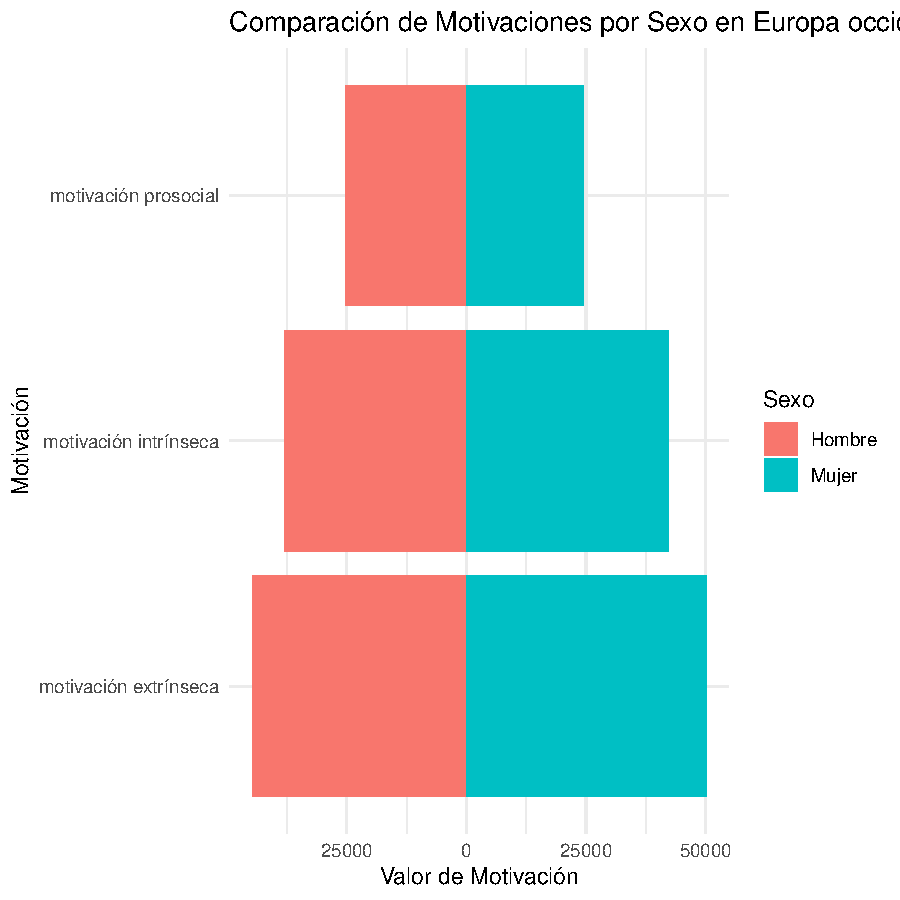
\includegraphics{Ejemplo-004}


\documentclass{article}
\usepackage{multicol}
\usepackage{booktabs} 
\usepackage{blindtext}
\usepackage{float}  

\renewcommand{\refname}{Referencias}
\renewcommand{\tablename}{Tabla}

\title{Ejemplo de Documento Sweave}
\author{Carlos Schmidt}
\date{2024-07-22}

\begin{document}


\maketitle

\textbf{Preguntas a las que este informe da respuesta:}
\begin{enumerate}
    \item ¿Cómo varían las tres motivaciones contempladas (extrínseca, intrínseca y prosocial) en función del sexo de los sujetos?
    \item ¿Cómo varían las tres motivaciones contempladas (extrínseca, intrínseca y prosocial) en función de la edad de los sujetos?
    \item ¿Cómo varían las tres motivaciones contempladas (extrínseca, intrínseca y prosocial) en función del nivel educativo de los sujetos?
    \item ¿Cuál es la distribución de los niveles de las tres motivaciones contempladas (extrínseca, intrínseca y prosocial) en los países de Europa occidental?
    \item ¿Cuál es la motivación principal de entre las tres contempladas (extrínseca, intrínseca y prosocial) en los países de Europa occidental?
\end{enumerate}



\section{Pregunta 2: ¿Cómo varían las tres motivaciones contempladas (extrínseca, intrínseca y prosocial) en función de la edad de los sujetos?}

En esta sección, realizaremos ANOVAs para comparar las medias de la motivación intrínseca, extrínseca y prosocial por categorías de edad.

